\section{Finishing comments}
We runned all the processes, get to know scheduling, get to know first come
first served algorithm. \\
There are upsides and downsides of first come first served algorithm:
\\
Upsides:
\begin{itemize}
	\item It is easy to implement
	\item It is easy to understand
\end{itemize}
Downsides:
\begin{itemize}
	\item It is very inefficient (Last experiment with 10 processes barely
		acknowledged existence of the 5th one)
	\item High average wait time (Imagine 1000 processes and how long we
		would have to wait)
\end{itemize}
Using pretty much any other algorithm we could get better results \cite{First
come first serve}
\begin{figure}[H]
	\caption{\href{https://commons.wikimedia.org/wiki/File:Process_states.svg}{[Process
	states and how they switch from wikimedia]}}
	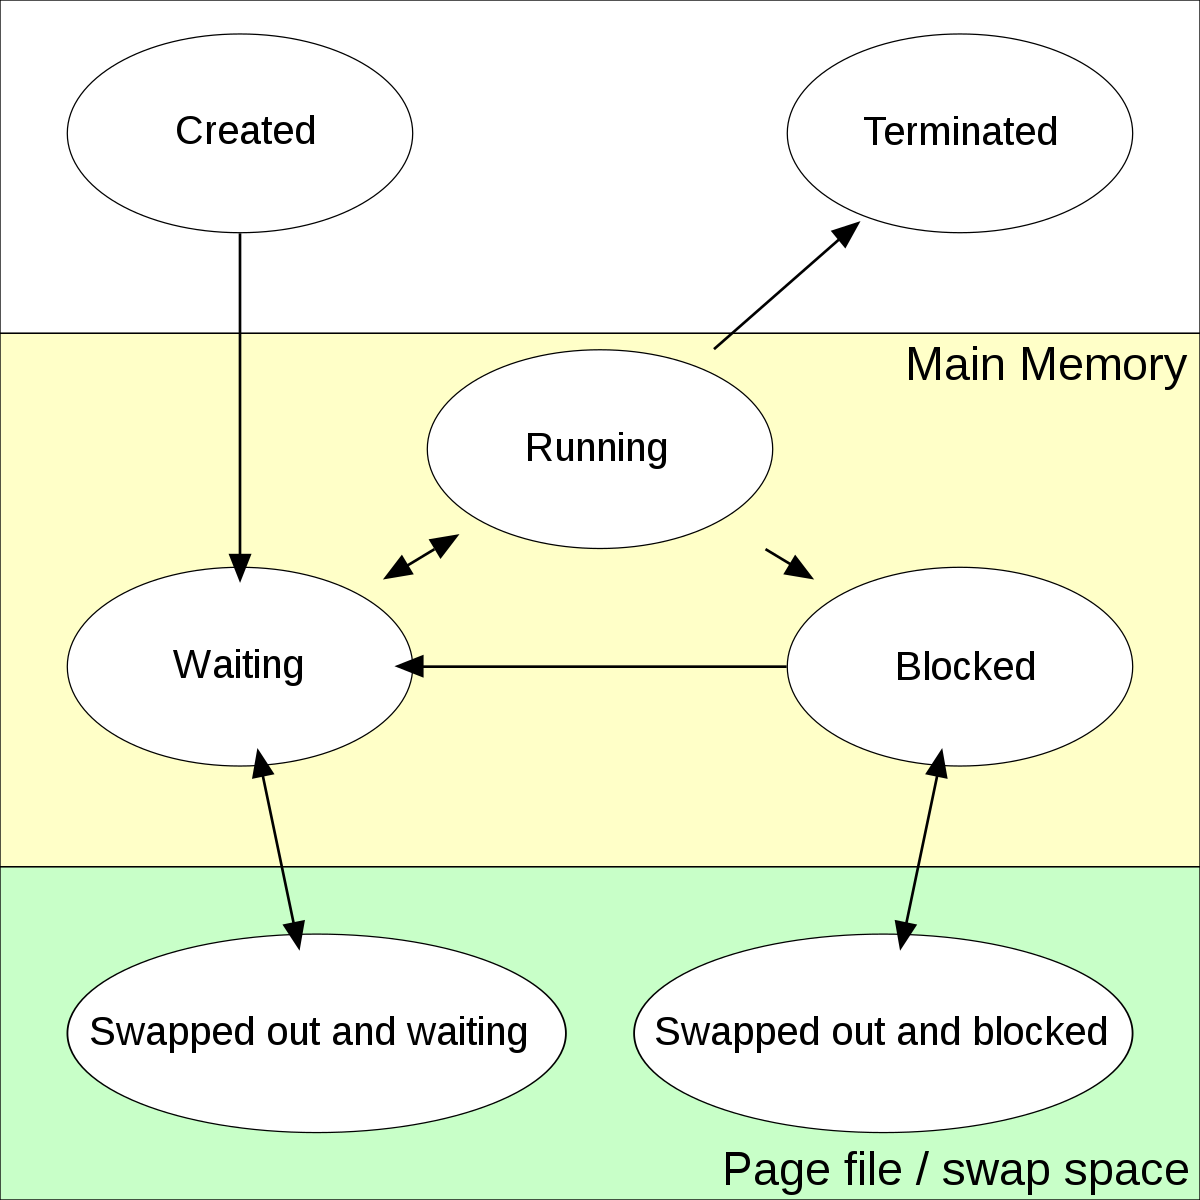
\includegraphics[width=\textwidth]{procestates}
\end{figure}

\begin{thebibliography}{9}
	\bibitem{lab3 Manual} Manual in the laboratory 3 files.
	\bibitem{First come first serve}
	\href{https://www.studytonight.com/operating-system/first-come-first-serve}{[https://www.studytonight.com/operating-system/first-come-first-serve]}
	\bibitem{Other scheduling algorithms}
	\href{https://www.tutorialspoint.com/operating_system/os_process_scheduling_algorithms.htm}{[Tutorials
point process scheduling algorithms]}
\end{thebibliography}
